\documentclass{article} % For LaTeX2e

%STANDARD PREAMBLE
%https://tex.stackexchange.com/questions/68821/is-it-possible-to-create-a-latex-preamble-header
\usepackage{/Users/mwojno01/Research/Learning/latex_preamble/preamble}

%%% 
% SPECIFIC TO THIS DOCUMENT
%%%

% SIGMA-FIELDS 
% Sigma fields (text)
\renewcommand{\sf}{$\sigma$-field}
\newcommand{\sfs}{$\sigma$-fields}


% SET FUNCTIONS 
%Finitely additive set functions
\newcommand{\fasf}{\tilde{\mu}_0}
% Signed measure
\newcommand{\signedmu}{\wt{\mu}}


% ENUMERATE BUT WITH LETTERS
\newenvironment{alphabate}
    {\begin{enumerate}[label=\alph*)]}
	{\end{enumerate} }
    
\begin{document}


\title{Notes on Probability and Measure Theory} 
\maketitle
\tableofcontents
\newpage 

\section{Overview}

\subsection{References}
The primary reference here is \cite{ash2000probability}.   The book is wonderful for statistical machine learning – it is rigorous,  but also accessible (prerequisites are undergrad-level real analysis and mathematical probability).  Most importantly, it is structured to build towards the kinds of applications in probability that we care about.   (A point of contrast would be a book like that of Stein and Shakarchi, which tends to dwell heavily on things that are of higher interest to pure mathematicians –- long existence proofs, Cantor sets and fractals, etc.) 

 Unless otherwise specified, all references to the ``text" refers to this textbook.  Likewise the symbol $\S$ refers to a Section of that textbook.
 
\subsection{Motivation} \label{sec:motivation}

Measure theory serves as a critical underpinning for some of the most interesting research in Bayesian statistics and probabilistic machine learning (see work from Stephen G. Walker, Michael Jordan, Tamara Broderick, David Dunson, and so on).   Thus, fluency with measure theory opens doors to a higher level of research consumption. 
  
Measure theory is convenient in unifying various kinds of random variables.\footnote{For example, it allows one to work with discrete and absolutely continuous random variables in a unified way.  For example, the exponential family includes both types of random variables.}  Lesbesgue integrals have nice limit theorems, and can be seen as the completion of Reimann integrals (in the same way that the real numbers complete the rationals). 



%We begin with a discussion of $\sigma$-fields, which are the domains of probability measures, and measures more generally.  As it turns out, measures cannot be defined on all subsets of many spaces that we would like to deal with. For instance, consider Proposition 1.2.6 of \cite{rosenthal2006first} which asserts the existence of non-measurable sets for the uniform distribution.  In particular, there is no definition of $P(A)$ that is defined for all subsets $A \subseteq [0,1]$ satisfying all three conditions below



\section{$\S$ 1.1: Some notes on set theory}

\subsection{Limits of sequences of sets}

\begin{definition}
The \textbf{upper limit} of a sequence of sets is given by
\[ \lim\sup A_n := \bigcap_{n=1}^\infty \bigcup_{k \geq n} A_k \]
Alternatively,
\[ x \in \lim\sup A_n \text{ iff } x \in A_n \text{ for infinitely many } n \]
\end{definition}

\begin{definition}
The \textbf{lower limit} of a sequence of sets is given by
\[ \lim\inf A_n := \bigcup_{n=1}^\infty \bigcap_{k \geq n} A_k \]
Alternatively,
\[ x \in \lim\inf A_n \text{ iff } x \in A_n \text{ eventually ( for all but finitely many $n$ ) } \]
\end{definition}

\begin{figure}
\centering 
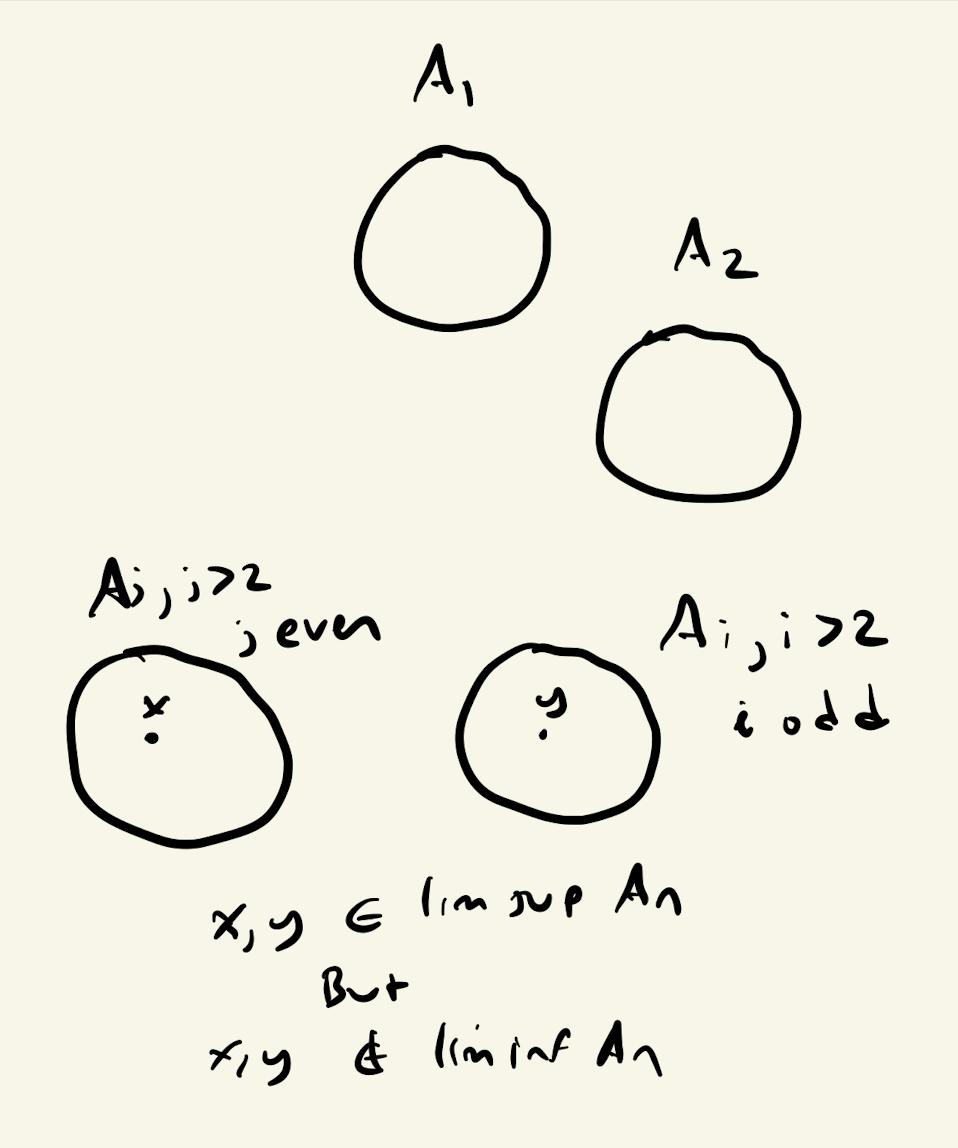
\includegraphics[width=.5\textwidth]{images/limsup_and_liminf}	
\caption{A sequence of sets with empty lower limit and non-empty upper limit.}
\end{figure}

\begin{discussion}
Discuss why the two characterizations of upper limit and lower limit are equivalent.	
\end{discussion}

\begin{definition}
If $\lim\inf A_n = \lim\sup A_n = A$, then A is called the \textbf{limit} of the sequence $A_1, A_2, ...$. 
\end{definition}

Now we present a particular kind of limit that will be useful when we discuss continuity of measure. 

\begin{definition}
If $A_1 \subset A_2 \subset ...$ and $\cup_{n=1}^\infty A_n = A$, we say that the $A_n$ form a \textbf{increasing} sequence of sets with limit $A$ or that the $A_n$ increase to $A$; we write $A_n \uparrow A$.  If $A_1 \supset A_2 \supset ... $ and  	$\cap_{n=1}^\infty A_n = A$, we say that the $A_n$ form a \textbf{decreasing} sequence of sets with limit $A$ or that the $A_n$ decrease to $A$; we write $A_n \downarrow A$.
\end{definition}


\begin{figure}[h!]
\centering 
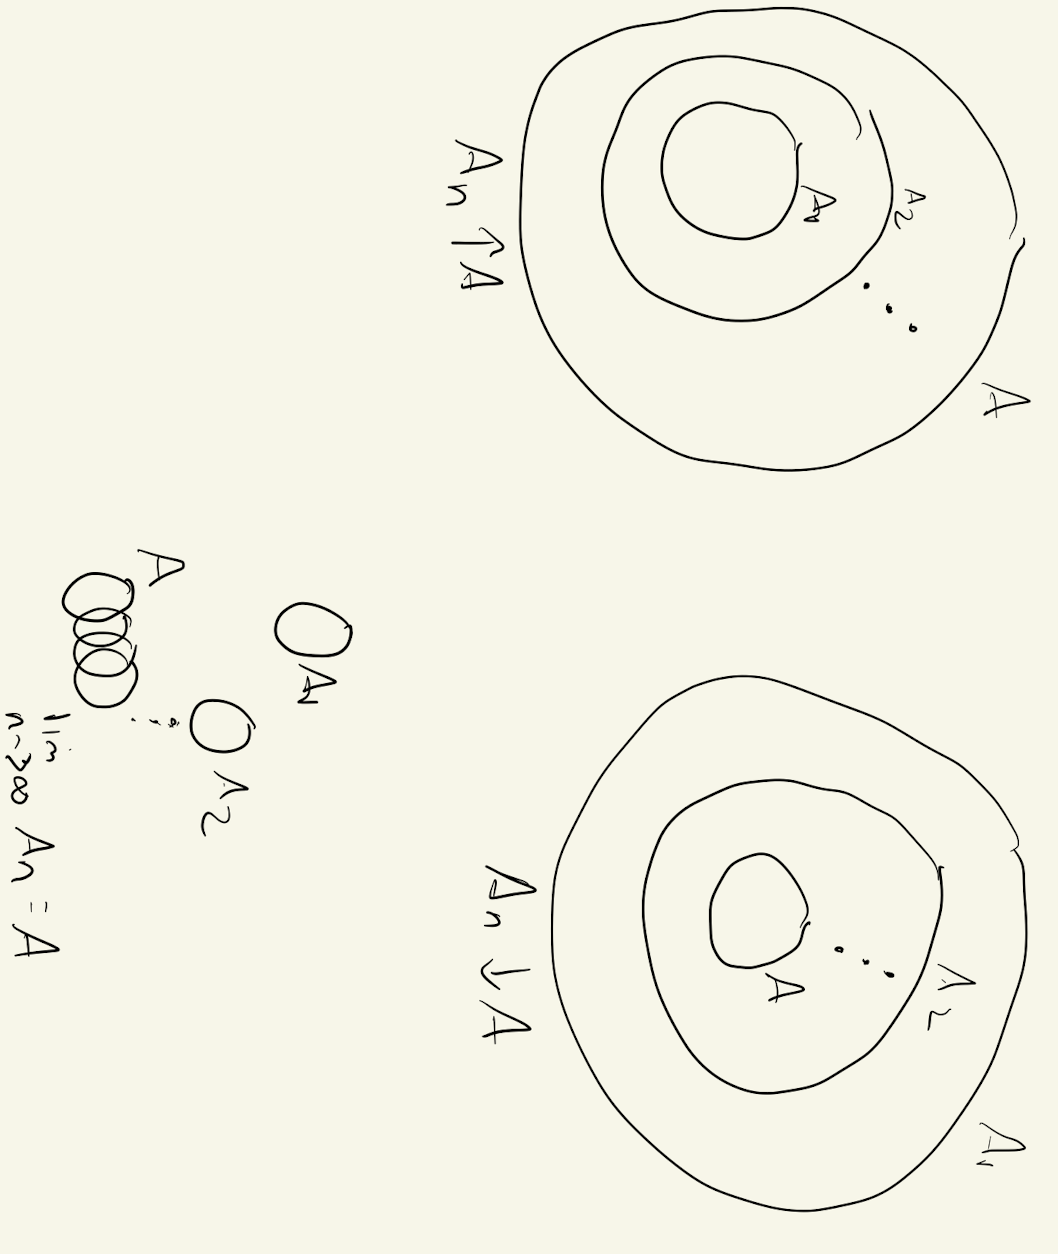
\includegraphics[width=.5\textwidth, angle=90]{images/increasing_and_decreasing_sequences}
\caption{An increasing and decreasing sequence of sets, followed by a sequence of sets which is neither, but which has a limit.}
\label{fig:increasing_and_decreasing_limits_of_sets}
\end{figure}

One can verify that this definition is consistent with the definition of limits, i.e.
\[  \text{If } A_n \uparrow A \text{ or } A_n \downarrow A \text{ then } \lim\inf A_n = \lim\sup A_n = A.\]

As shown in Figure \ref{fig:increasing_and_decreasing_limits_of_sets}, limits of increasing and decreasing sequences are very special kinds of limits.


\subsection{Representing unions as disjoint unions}
 
\begin{remark}
If $A_1,A_2,...$ are subsets of some set $\Omega$, then
\begin{align*} 
\bigcup_{n=1}^\infty A_n = \bigcupdot_{n=1}^\infty \bigg(A_n \cap A_{n-1}^c \cap ... \cap A_1^c \bigg) 	
\labelit \label{eqn:union_as_disjoint_union}
\end{align*}

In other words, any union can be re-represented as a disjoint union. This is useful because measures are countably additive on disjoint sets, so we prefer to work with collections of disjoint sets.
\label{rk:rerepresenting_unions_as_disjoint_unions}
\end{remark}

\begin{remark}
If $A_n \uparrow A$, then \eqref{eqn:union_as_disjoint_union} becomes
\begin{align*}
	\bigcup_{n=1}^\infty A_n = \bigcupdot_{n=1}^\infty \bigg( A_n - A_{n-1} \bigg) 
\labelit \label{eqn:union_as_disjoint_union_for_increasing_sequences}
\end{align*}
This is because $A_{n-1} \subset A_{n}$, so $A_{n-1}^c \supset A_{n}^c$ by contraposition.	
\end{remark}

\section{$\S$ 1.2: Fields, \sfs, measures}

\subsection{$\S$ 1.2.1-1.2.2: Fields and \sfs}

Probability measures, and measures more generally, cannot be defined on all subsets of many spaces that we would like to deal with.  For instance, non-measurable sets can be shown to exist even for Lesbesgue measure on the unit interval.  Proposition 1.2.6 of \cite{rosenthal2006first} shows that there is no definition of $P(A)$ that is defined for all subsets $A \subseteq [0,1]$ satisfying all three conditions below
\begin{enumerate}
\item $P([a,b]) = b-a, \quad 0 \leq a \leq b \leq 1$.	
\item $P(\bigcupdot_{n=1}^\infty A_n ) = \ds\sum_{n=1}^\infty A_n$ for $A_1, A_2, ...$ disjoint subsets of $[0,1]$.
\item $P(A \bigoplus r) = P(A), \quad 0 \leq r \leq 1$, where $A \bigoplus r$ denotes the \textit{r-shift} of $A$, i.e. 
\[ A \bigoplus r := \set{a+r : a \in A, a+r \leq 1} \cup \set{a+r-1 : a \in A, a +r >1}\]
\end{enumerate}

The solution to this problem is to define measures on a restricted domain, $\sigma$-fields.

\subsubsection{$\sigma$-fields}



%We begin with a discussion of $\sigma$-fields, which are typically the domains of probability measures, and measures more generally.\footnote{In the construction of Lesbesgue measure, Ash defines a probability measure on a field.  See 1.3.1 of \cite{ash2000probability}.}  As stated in the motivation (Section \ref{sec:motivation}), measures cannot be defined on all subsets of many spaces that we would like to deal with. 

%\sfs\ are important because they are the domain of measures.  
%Here are some definitions.

\begin{definition}
Let $\F$ be a collection of subsets of a set $\Omega$.  Then $\F$ is called a \textbf{sigma-field} (or \textit{sigma-algebra}) if it satisfies

\begin{enumerate}[label=\alph*)]
	\item $\Omega \in \F$ 
	\item If $A \in \F$, then $A^c \in \F$.
	\item If $A_1,A_2, ... \in \F$ then $\cup_{i=1}^\infty A_i \in \F$.  
\end{enumerate}
that is, if $\Omega \in \F$ and $\F$ is closed under complementation and countable unions.
\label{def:sigma_field}	
\end{definition}

\begin{remark}
It follows that $\sigma$-fields are closed under countable intersections, since
\[ \cap_{i=1}^\infty A_i \stackrel{\text{DeMorgan's Law}}{=} \cup_{i=1}^\infty A_i^c \]	
\end{remark}

\begin{example}
$\F =\set{\emptyset, \Omega}$ is the smallest \sf\ on $\Omega$. 
\end{example}

\begin{example}
	$\F =2^\Omega$, i.e. the set of all subsets of $\Omega$, is the largest \sf\ on $\Omega$.
\end{example}

\begin{example}
If $A \in \Omega$ is non-empty, then $\F = \set{\emptyset, A, A^c, \Omega}$ is the smallest \sf\ containing $A$.
\end{example}

\begin{notation}
If $\C$ is a class of sets, the smallest \sf\ containing the sets of $\C$ is written as $\sigma(\C$).  This is sometimes called the \textit{minimal \sf\ over $C$} or the \textit{\sf\ generated by $C$}. 
\end{notation}
	
\begin{exercise}
\label{exercise:minimal_sigma_field_containing_n_subsets}
Let $A_1,...,A_n$ be subsets of $\Omega$.  Describe $\F := \sigma(\set{A_1,...,A_n})$, the smallest \sf\ containing $A_1,...,A_n$.  Also describe the number of sets in $\F$.   \textit{This is Ash's Problem 1.2.8.  We can derive the strict upper bound $|\F| \leq 2^{2^n}$. For a complete answer, see GoodNotes. }	
\end{exercise}

\begin{remark}
The gist of exercise \ref{exercise:minimal_sigma_field_containing_n_subsets} is that the collection $\set{A_1,...,A_n}$ partitions $\Omega$ into up to $M=2^N$ pieces, and the minimal sigma field contains all possible finite unions of these pieces, so has at most $2^{M}$ elements.
  
\begin{figure}[h!]
\centering 
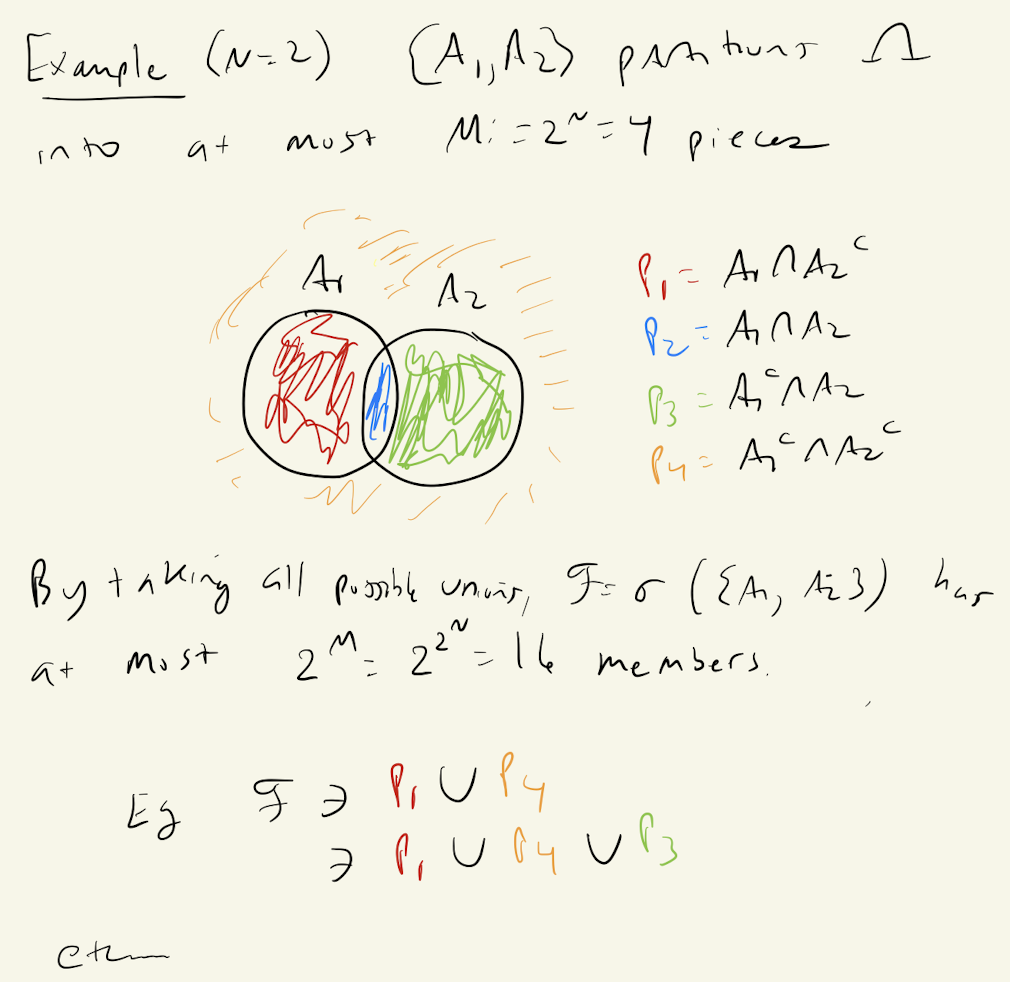
\includegraphics[width=.7\textwidth]{images/minimal_sigma_fields}
%\caption{An increasing and decreasing sequence of sets, followed by a sequence of sets which is neither, but which has a limit.}
\end{figure}

\end{remark}

\subsubsection{Fields}

Fields are more general than $\sigma$-fields.  Measures are sometimes constructed by being defined on fields, and then extended to \sfs.  Indeed, we will see this strategy with Lesbesgue measure. 

\begin{definition}
Let $\F$ be a collection of subsets of a set $\Omega$.  Then $\F$ is called a \textbf{field} (or \textit{algebra})  if satisfies Definition \ref{def:sigma_field} after replacing condition c) with

\begin{enumerate}
	\item[c')] If $A_1,...A_n \in \F$ then $\cup_{i=1}^n A_i \in \F$.
\end{enumerate}
that is, if $\Omega \in \F$ and $\F$ is closed under complementation and \textit{finite} unions.
\label{def:field}	
\end{definition}

\begin{example} What is an example of a collection that is a \textit{field}, but not a $\sigma$-\textit{field}?  

Let $\Omega=\R$ and $\F_0 = \set{\text{finite disjoint unions of right semi-closed intervals } (a,b], a \neq b}$.  Then $\F_0$ is a field, as can be easily verified.\footnote{By convention, we also count $(a, \infty)$ as right semi-closed for $-\infty\leq a < \infty$, which is necessary for the \sf\ to be closed under complements.}   

\begin{figure}[h!]
\centering
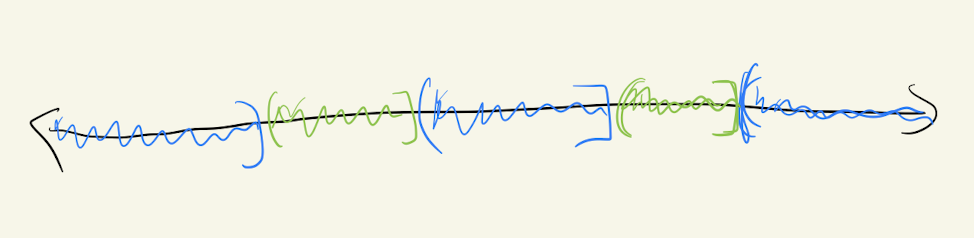
\includegraphics[width=.6\textwidth]{images/rsc_intervals}	
\end{figure}

But $\F_0$ is \underline{not} a \sf.  Note that if $A_n = (-\frac{1}{n},0]$, then $\bigcap_{n=1}^\infty A_n = \set{0}  \not\in \F_0$.
\label{ex:field_of_finite_disjoint_unions_of_rsc_intervals}
\end{example}

\begin{remark}
A \sf\ can also be described as a field that is closed under limits of increasing sequences.  For if $A_n \in \F$ and $A_n \uparrow A$, then A is a countable union of sets in $\F$ by definition.  Conversely, if $A = \cup_{n=1}^\infty A_n$, then set $B_N := \cup_{n=1}^N A_n$ and $B_N \uparrow A$.	So if $\G$ is the collection of all limits of increasing sequences of sets in some field $\F_0$, we can also describe $\G$ as the collection of all countable unions of sets in $\F_0$. \label{rk:the_limits_of_increasing_and_decreasing_sequences_of_sets_in_a_field_are_also_the_countable_unions}
\end{remark}
%Recalling Figure \ref{fig:increasing_and_decreasing_limits_of_sets}, limits of increasing sequences are very special kinds of limits.


\subsubsection{``Good sets" strategy} \label{sec:good_sets_strategy}

Ash says that there is a type of reasoning that occurs so often in problems involving \sfs\ that it deserves explicit mention.  It is called the \textit{good sets strategy}.   Suppose you want to show that all members of a $\sigma$-algebra   $\F$ have some property $P$.  Define ``good sets" as those that satisfy the property
\[ \G := \{ G \in \F : G \text{ has property } P \} \]
The strategy is then to simply
\begin{enumerate}
\item Show $\G$ is a $\sigma$-algebra 
\item Show $\G$ contains some class $\C$ such that $\F = \sigma(\C)$	
\end{enumerate}


Then you're done!  

Why does this work?

\begin{align*}
& \quad \C \subset \G &&	\text{by 2}\\
&\implies \sigma(\C) \subset \sigma(\G) &&  \\
&\implies \F \subset \G && \text{by 1,2} \\
& \text{Yet $\G \subset \F$ by definition of $\G$.} && \\
& \text{So $\G = \F$.} && \\
& \text{ So all sets in $\F$ are good.} && \\
\end{align*}

Some example applications:
 \begin{itemize}
 \item In the text, Ash uses this strategy (see pp.5) to show that if $\C$ is a class of subsets of $\Omega$, and $A \in \Omega$, then

\[ \explaintermbrace{take minimal sigma field first, then intersect}{\sigma_\Omega(\C) \cap A} = \explaintermbrace{intersect first, then take minimal sigma-field}{\sigma_A(\C \cap A)} \]
 \item  See my handwritten homework exercise for  $\S$ 1.2, Problem 6.
 \item See the proof of Caratheodory Extension Theorem (Theorem \ref{thm:caratheodory_extension}).	
 \end{itemize}


\subsection{$\S$ 1.2.3-1.2.4: Measures}




\begin{definition}
A \textbf{measure} on a \sf\ $\F$ is a non-negative, extended real-valued function $\mu$ on $\F$ such that whenever $A_1, A_2, ...$ form a finite or countably infinite collection of disjoint sets in $\F$, we have countable additivity; that is,
\[ \mu \bigg( \bigcupdot_n A_n \bigg) = \ds\sum_n \mu(A_n) \]
\label{def:measure}	
\end{definition}

\begin{definition}
A \textbf{probability measure} is a measure (Definition \ref{def:measure}) where $\mu(\Omega)=1$.
\label{def:prob_measure}		
\end{definition}

\begin{remark}
Ash additionally assumes that a measure does not take $\mu(A) = \infty$ for all $A \in \F$.\footnote{Likewise, he assumes that signed measures do not take $\mu(A) = -\infty$ for  for all $A \in \F$.}  From this, we automatically obtain $\mu(\emptyset)=0$. For $\mu(A) < \infty$ for some $A$, and by considering the sequence $A, \emptyset, \emptyset, ...$, we have that $\mu(\emptyset)=0$ by countable additivity.   	
\end{remark}

\begin{example}
Let $\Omega$ be any set.  Fix $x_0 \in \Omega$.  Let $\F = 2^\Omega$.  For any $A \in \F$ define $\mu(A) = 1$ if $x_0 \in A$ and $\mu(A) = 0$ if $x_0 \not\in A$.  Then $\mu$ may be called the \textbf{unit mass} concentrated at $x_0$.
\end{example}

\begin{example}
Let $\Omega = \set{x_1,x_2,...}$ be a finite or countably infinite set.  Let $p_1, p_2,...$ be non-negative reals.  Let $\F = 2^\Omega$.  Define
\[\mu(A) = \ds\sum_{x_i \in A} p_i \quad \text{ for all } A \in \F\]
Then $\mu$ is a measure on $\F$. We might call it the ``point weighting" measure. 
\begin{itemize}
\item If $p_i \equiv 1 \; \forall \, i$, then $\mu$ is called the \textbf{counting measure}.
\item If $\sum_i p_i =1$, then $\mu$ is a probability measure.	
\end{itemize}
	
\end{example}


\begin{example}{\remarktitle{Lesbesgue measure}}
Define $\mu$ such that 
\[ \mu(a,b] = b-a \quad \forall \, a,b \in \R : b>a \]
As we will see in Section \ref{sec:extension_of_measures}, this requirement determines $\mu$ on a large collection of sets, the Borel Sets $\B(\R)$, defined as the smallest \sf\ of subsets of $\R$ containing all intervals $(a,b] \subset \R$.

We may alternately characterize $\B(\R)$ as the smallest \sf\ containing
\begin{itemize}
\item all intervals $(a,b], \; a,b \in \R$
\item all intervals $(a,b), \; a,b \in \R$
\item all intervals $[a,b), \; a,b \in \R$
\item all intervals $[a,b], \; a,b \in \R$.
\item all intervals $(a,\infty), \; a \in \R$.
\item  all intervals $[a,\infty), \; a \in \R$.
\item 	 all intervals $(-\infty,b), \; b \in \R$.
\item  all intervals $(-\infty,b], \; b \in \R$.
\item all open sets of $\R$.\footnote{Recall that an open set is a countable union of open intervals.}
\item all closed sets of $\R$.\footnote{Recall that a set is open iff its complement is closed.}
\end{itemize}

To illustrate these equivalences, let us equate the first two conditions. That is, let us show that a \sf\ contains all open intervals $(a,b)$ iff it contains all right semi-closed intervals $(a,b]$.  To see this, simply note

\begin{align*}
(a,b] &= \bigcap_{n=1}^\infty \bigg(a, b+\frac{1}{n}\bigg) \\
	\intertext{and}
(a,b) &= \bigcup_{n=1}^\infty \bigg(a, b-\frac{1}{n}\bigg] 
\end{align*}
\label{ex:lesbesgue_measure}
\end{example}

\begin{question}
The text gives another description of the Borel sets $\B(\R)$ as the smallest \sf\ containing $\F_0$, the field of disjoint unions of right semi-closed intervals $(a,b]$.  Can we make the same statement about the field of finite disjoint unions of left semi-closed intervals?
\end{question}

\subsection{$\S$ 1.2.5-1.2.6: Properties of measures (and some more general set functions)}

The text considers some generalizations of measures that can be obtained
\begin{enumerate}
\item  by restricting the domain to a field {\footnotesize (in other texts, such functions are called \textit{pre-measures}) }
\item  by only assuming \textit{finite} additivity 
\item by allowing the range to be extended reals ($\bar{\R}$) instead of non-negative extended reals ($\bar{\R}_{\geq 0}$).  
\end{enumerate}



\begin{remark}
With respect to pre-measures, a countably additive function can be defined on a \textit{field} (rather than \sf) if the condition is taken to hold whenever a countable union \textit{does} happen to still be in the field.  Unless otherwise specified, I will assume in these notes by that countably additive functions are always defined on \sfs, and finitely additive functions are defined on fields.
\label{rk:i_am_assuming_a_domain_based_on_the_type_of_additivity}
\end{remark}	



\begin{table}[!h]
\centering	
\begin{tabular}{rcc}
&\multicolumn{2}{c}{\textbf{Range}} \\
& \textbf{non-negative extended reals} & \textbf{extended reals} \\
\textbf{countably additive}& $\mu$ measure  & $\tilde{\mu}$ signed measure \\
\textbf{finitely additive}& $\mu_0$ & $\tilde{\mu}_0$ \\	
\end{tabular}
\caption{Notation for generalizations of measure (For assumed domain in each case, see Remark \ref{rk:i_am_assuming_a_domain_based_on_the_type_of_additivity}.)}
\label{tab:notation_for_generalizations_of_measure}
\end{table}

In Table \ref{tab:notation_for_generalizations_of_measure},  we introduce some notation to try to clarify more immediately when results hold. Note the relations\footnote{So, for example, if something holds for $\tilde{\mu}_0$, it holds for $\mu$.  A simple mnemonic is that adding stuff to the notation generalizes the function.}  
\[ \set{\mu} \subset \set{\mu_0}, \set{\tilde{\mu}} \subset \set{\tilde{\mu}_0}. \]

\begin{remark}
Being able to work with these generalizations will be important in Section \ref{sec:extension_of_measures} on extension of measures.  In particular, it will help us show that we can construct the Lesbesgue measure on the Borel sets.
\end{remark}

 \begin{example} Let $\F_0$ be the field of finite disjoint unions of right semi-closed intervals (see Definition \ref{def:rsc_intervals} ), and define the set function $\fasf$ on $\F_0$ as follows\footnote{This example comes from Problem 4 in Section 1.2 of the text}:

\begin{align*}
\fasf(-\infty,a] &=a, && a \in \R  \\
\fasf(a,b] &= b-a, && a,b \in \R, \quad a<b  \\
\fasf(b, \infty) &= -b, && b \in \R \\
\fasf(\R) &=0 &&\\
\fasf(\bigcupdot_{i=1}^n I_i) &= \sum_{i=1}^n \fasf(I_i), && \text{if $I_1, ..., I_n$ are right semi-closed intervals} 
\end{align*}
	
Then $\fasf$ is finitely additive, but not countably additive on $\F_0$.  (Why?) For a proof, see GoodNotes.
 \end{example}

 
Measure-like set functions have useful properties. Using the notation in Table \ref{tab:notation_for_generalizations_of_measure}, we rewrite Theorem 1.2.5 of the text:
 
 \begin{theorem}
 Let $\fasf$ be a finitely additive set function on the field $\F_0$.  Then
 \begin{enumerate}[label=\alph*)]
 \item \label{itm:first} $\fasf(\emptyset)=0$
 \item \label{itm:second} $\fasf(A \cup B) + \fasf (A \cap B) = \fasf(A) + \fasf(B)$ for all $A,B \in \F_0$.
 \begin{figure}[H]
 \centering
 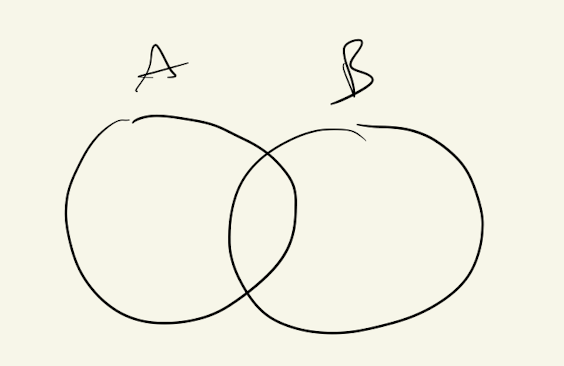
\includegraphics[width=.2\textwidth]{images/two_overlapping_sets}	
 \end{figure}

 \item \label{itm:piece-and-difference} If $A,B \in \F_0$ and $B \subset A$, then   
  \[ \fasf(A) = \fasf(B) + \fasf(A-B)\quad \text{(piece-and-difference decomposition)} \] 
 \begin{figure}[H]
 \centering
 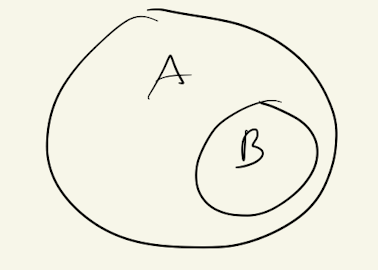
\includegraphics[width=.2\textwidth]{images/whole_and_piece}	
 \end{figure}
 
 \footnote{If the ``piece" satisfies $\fasf(B) < \infty$, we have $\fasf(A-B) = \fasf(A) - \fasf(B) $.  One useful takeaway for piece-and-difference decompositions is that : \textit{the finite measure of the difference is the difference of the finite measures}.}So $\fasf(A) \geq \fasf(B)$ if $\fasf(A-B) \geq 0$. More generally, for non-negative set functions, we have
 \[ \mu_0 (A) \geq \mu_0 (B) \quad \text{(monotonicity)} \] 
 \item \label{itm:subadditivity} Subadditivity holds if $\fasf$ is non-negative, i.e.
 \begin{align*}
 \mu_0 (\cup_{i=1}^n A_i)& \leq \sum_{i=1}^n \mu_0(A_i) \\
  \mu (\cup_{i=1}^\infty A_i)& \leq \sum_{i=1}^\infty \mu(A_i) \\
 \end{align*}
 \end{enumerate}
\label{thm:basic_properties_of_finitely_additive_set_functions}
 \end{theorem}
  
\begin{proof}
 We prove Theorem \ref{thm:basic_properties_of_finitely_additive_set_functions} (b).  The rest is an exercise for the reader (or see the text).
 
 First, we break things into disjoint pieces
 {\footnotesize 
\begin{align*}
A &= \bigg(A \cap B \bigg) \, \bigcupdot \, \bigg(A \cap B^c \bigg)	&& \implies \fasf(A) = \fasf (A \cap B) +  \fasf (A \cap B^c)  && (1) \\
B &= \bigg(A \cap B \bigg) \, \bigcupdot \, \bigg(A^c \cap B \bigg)	&& \implies \fasf(B) = \fasf (A \cap B) +  \fasf (A^c \cap B)  && (2) \\
A \cup B &= \bigg(A \cap B \bigg) \, \bigcupdot \, \bigg(A \cap B^c \bigg) \bigcupdot \, \bigg(A^c \cap B \bigg)	&& \implies \fasf(A \cup B) = \fasf (A \cap B) +  \fasf (A \cap B^c) + \fasf (A^c \cap B)   && (3) 
\end{align*}
}

Summing (1) and (2), we obtain
\[\fasf(A) + \fasf(B) = 2 \fasf(A \cap B) + \fasf(A \cap B^c) + \fasf(A^c \cap B). \]
We use (3) to simplify the RHS, and the result follows.
\end{proof}

\begin{remark}
In the proof of Theorem \ref{thm:basic_properties_of_finitely_additive_set_functions} (b), note that we use a common strategy -- breaking sets into disjoint pieces so that we can apply the assumed (finite or countable) additivity of the set function. 
\end{remark}


\begin{remark}
Is \textit{finiteness} ($|\mu_g (A)| < \infty \; \forall \; A \in \F_g$) equivalent to \textit{boundedness} ($\sup \set{|\mu_g (A)| : A \in \F_g} < \infty$)?
\begin{itemize}
\item $\mu_0, \signedmu$ ? \greencheck
\item $\fasf$ ? \redx (too general)
\end{itemize}
The fact that equivalence holds for signed measures $\signedmu$ is surprising.  Somehow countable additivity compensates for the signedness. See Section 2.1.3 of the text. 
\end{remark}


\subsection{$\S$ 1.2.7-1.2.8: Continuity of countably additive set functions}

Countably additive set functions have a basic continuity property. Continuity of measure is a special case. 

\begin{theorem}
Let $\signedmu$ be a countably additive set function on the \sf\ $\F$. Then

\begin{alphabate}
\item (continuity from below) If $A_1, A_2, ... \in \F$ and $A_n \uparrow A$, then $\signedmu(A_n) \to \signedmu(A)$ as $n \to \infty$.

\begin{figure}[H]
 \centering
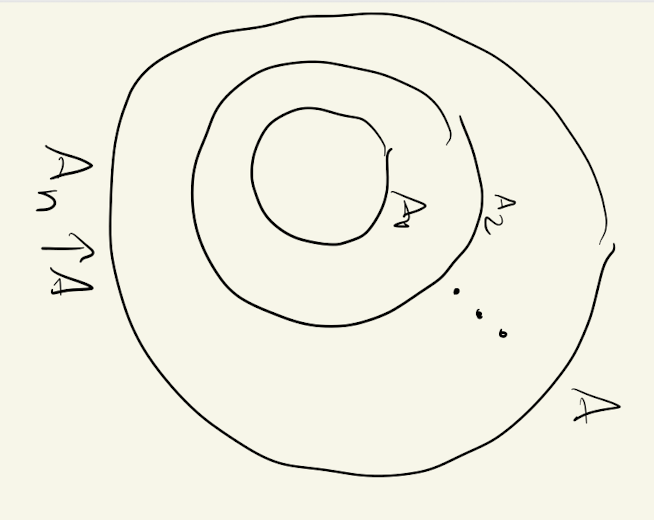
\includegraphics[width=.2\textwidth, angle=90]{images/increasing_sequence_of_sets}	
 \end{figure}
   
\item (continuity from above)  If $A_1, A_2, ... \in \F$, $A_n \downarrow A$, and $\signedmu(A_1)$ is finite, then $\signedmu(A_n) \to \signedmu(A)$ as $n \to \infty$. 
\end{alphabate}
\label{thm:continuity_of_countably_additive_set_functions}
\end{theorem}

\begin{proof}
We prove continuity from below, and leave continuity from above as an exercise to the reader (or see text). 
 
First let us assume that all $\signedmu(A_n)$ are finite (*). Then 
\begin{align*}
A &= A_1 \cupdot (A_2 - A_1) \cupdot (A_3 - A_2) \cupdot ... && 	\text{ by } \eqref{eqn:union_as_disjoint_union_for_increasing_sequences} \\
\implies \signedmu(A) &= \signedmu(A_1) + \signedmu(A_2 - A_1) + \signedmu(A_3 - A_2) + ... && \text{(countable additivity)}\\ 
&= \signedmu(A_1) + \signedmu(A_2) - \signedmu(A_1) + \signedmu(A_3) - \signedmu(A_2) + ... && \text{(Theorem \ref{thm:basic_properties_of_finitely_additive_set_functions} \ref{itm:piece-and-difference}, (*) }\\
&= \ds\lim_{n \to \infty} \signedmu(A_n) && \text{(telescoping difference)}
\end{align*}
Now suppose $\signedmu(A_n) = \infty$ for some $n$.   So write 
\begin{align*}
A &= A_n \cupdot A- A_n && \text{(increasing sequence)}\\ 
\implies \signedmu(A) &= \signedmu(A_n) + \signedmu(A - A_n) && \text{(countable additivity)}\\  
&= \infty + \signedmu(A - A_n) 
\end{align*}

So $\signedmu(A)=\infty$.\footnote{Note that we cannot have $\signedmu(A - A_n)=-\infty$, because that would violate additivity.} Replace $A$ by $A_k$ for any $k \geq n$ to also find $\signedmu(A_k)=\infty$ for all $k \geq n$ and the result follows.

Finally suppose $\signedmu(A_n) = -\infty$ for some $n$. Then the result follows in the same way as for $\signedmu(A_n) = \infty$. 

\end{proof}

\begin{remark}
The logic of the proof of Theorem \ref{thm:continuity_of_countably_additive_set_functions} under the finiteness assumption is as follows.  First, we re-represent the union as a disjoint union (the form is particularly simple since the sets are increasing).  This allows us to apply countable additivity. Then we apply the piece-and-difference decomposition (and the subtraction is defined under the finiteness assumption). 	
\end{remark}

\begin{remark}
In proving Theorem \ref{thm:continuity_of_countably_additive_set_functions}  for the case where $\mu(A_n) = \infty$ for some $n$, it is tempting to make the simpler argument 
\begin{align*}
\mu(A) & \geq \mu(A_n) && \text{(monotonicity)}\\	
\mu(A_k) & \geq \mu(A_n) && \text{(monotonicity)}	 
\end{align*}
for $k \geq n$.  But recall from Theorem \ref{thm:basic_properties_of_finitely_additive_set_functions} that monotonicity only holds under non-negativity, and the theorem statement is more general, applying to \textit{signed} set functions as well. 
\end{remark}

We have the result that finite additivity plus continuity equals countable additivity. 

\begin{theorem}
Let $\fasf$ be a finitely additive set function on the field $\F_0$.  Suppose either
\begin{alphabate}
\item $\fasf$ is continuous from below
\item $\fasf$ is continuous from above at the empty set.	
\end{alphabate}
Then $\fasf$ is countably additive.
\label{thm:finite_additivity_plus_continuity_gives_countable_additivity}
\end{theorem}

\begin{proof}
We prove that the conclusion holds under (a) and leave doing the same for (b) as an exercise to the reader (or see text). 	%To show that $\fasf$ is countably additive, we need to show that  $ \fasf \bigg( \bigcupdot_{n=1}^\infty A_n \bigg) = \ds\sum_{n=1}^\infty \fasf(A_n)$.   

Given $A = \bigcupdot_{n=1}^\infty A_n$, we define $P_n := \bigcup_{m \leq n} A_n$ and so $P_n \uparrow A$.   So we have
\begin{align*}
\fasf(P_n) &\to \fasf(A) && \text{(continuity from below)} \\
\implies \fasf(\bigcup_{m \leq n} A_n) &\to \fasf(A) && \text{(definition)} \\	
\implies \ds\sum_{m=1}^n \fasf(A_n) &\to \fasf(A) && \text{(finite additivity)} \\
\end{align*}
Taking $n \to \infty$ gives countable additivity.
\end{proof}





%By , we have


 %we break up the limit of the increasing sequence into a disjoint union as follows	



 \section{$\S$ 1.3: Extension of measures} \label{sec:extension_of_measures}
 
 
\subsection{Extension and approximation} \label{sec:extension_and_approximation}
 
In Example \ref{ex:lesbesgue_measure}, we discussed the concept of length of a subset of $\R$; in particular, we mentioned extending the set function given on intervals by $\mu(a,b] = b-a$ to a larger class of subsets of $\R$.  


 As remarked in Example \ref{ex:field_of_finite_disjoint_unions_of_rsc_intervals}, if we define $\F_0 = \set{\text{finite disjoint unions of right semi-closed intervals } (a,b], a \neq b}$, then $\F_0$ is a field, as can be easily verified.  And $\mu$ can easily be seen to be a finitely additive set function on $\F_0$.   

\begin{figure}[H]
\centering
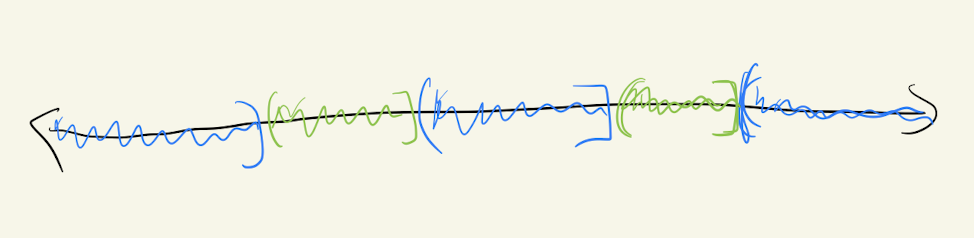
\includegraphics[width=.6\textwidth]{images/rsc_intervals}	
\end{figure}

However, $\F_0$ is not a $\sigma$-field.  So how can we extend this function to a measure on a larger class of subsets?  The challenges are:

\begin{itemize}
\item \textit{We need to show that $\mu$ is countably additive.} We will do this in Section 5.   Moreover, in that section, we will generalize our problem to set functions given by $\mu(a,b] = F(b)-F(a)$, where $F$ is an increasing right-continuous function from $\R$ to $\R$.
\item \textit{We need to extend $\mu$ to $\sigma(\F_0)$, the minimal $\sigma$-field containing $\F_0$.} In other words, we need to extend $\mu$ to the Borel sets.  We will handle the problem in this section more generally.  In this section, we will deal with the problem of extending a measure on $\F_0$ to a measure on $\sigma(\F_0)$. We do so using Carath\'eodory's Theorem  (Theorem \ref{thm:caratheodory_extension}).  Along the way, we will use Theorem \ref{thm:extension_of_finite_measure} and Theorem \ref{thm:monotone_class_theorem} to prove Theorem \ref{thm:caratheodory_extension}. 
% We refer to a countably additive set function $\mu$ on a field $\F_0$ as a \textit{pre-measure}
\end{itemize}

 \begin{theorem}
 (Theorem 1.3.6 \cite{ash2000probability}) A finite measure on a field $\F_0$ can be extended to a measure on $\sigma(\F_0)$. 	
 \label{thm:extension_of_finite_measure}
 \end{theorem}

\begin{proof}
See pp. 12-17 of \cite{ash2000probability}.	
\end{proof}

\begin{theorem}{\textbf{(Monotone Class Theorem)}}
Let $\F_0$ be a field of subsets of $\Omega$ and $\C$ be a class of subsets of $\Omega$ that is monotone (if $A_n \in \C$ and $A_n \uparrow 
A$ or $A_n \downarrow A$, then $A \in \C$).  If $\C \supset \F_0$ then $\C \supset \sigma(\F_0)$, then minimal $\sigma$-field over $\F_0$. 
 \label{thm:monotone_class_theorem}
\end{theorem}

\begin{proof}
See pp. 18-19 of \cite{ash2000probability}.	
\end{proof}

\begin{remark}
During the proof of Theorem \ref{thm:monotone_class_theorem}, some key observations are made about the relationship between monotone classes and $\sigma$-fields:
\begin{alphabate}
\item A monotone class that is also field is a sigma-field.  (See Remark \ref{rk:the_limits_of_increasing_and_decreasing_sequences_of_sets_in_a_field_are_also_the_countable_unions}.)
\item The smallest monotone class and smallest sigma-field over a field coincide. 
\end{alphabate}
\label{rk:monotone_classes_and_sigma_fields}
\end{remark}

\begin{theorem}{\textbf{(Carath\'eodory Extension Theorem)}} Let $\mu$ be a measure on the field $\F_0$ of subsets of $\Omega$, and assume that $\mu$ is $\sigma$-finite on $\F_0$, so that $\Omega$ can be decomposed as $\cup_{n=1}^\infty A_n$ where $A_n \in \F_0$ and $\mu(A_n) < \infty$ for all $n$.  Then $\mu$ has a unique extension to a measure on $\F := \sigma(\F_0)$, the minimal $\sigma$-field over $\F_0$. 
 \label{thm:caratheodory_extension}
\end{theorem}

\begin{proof} (We follow the argument of \cite{ash2000probability}, but add some detail.) 
First we prove existence.  {\footnotesize [Without loss of generality, we assume the $A_n$ are disjoint.  This is possible because we can use \eqref{eqn:union_as_disjoint_union} to re-express the countable union as a disjoint countable union:  $\Omega = \cup_{i=1}^\infty A_i = \cupdot_{i=1}^\infty B_i$, where $B_i := A_i \cap A_{i-1}^c ... \cap A_1^c$.]  } 

If we define $\mu_n(A)=\mu(A \cap A_n)$ for each $A \in \F_0$, then we can decompose $\mu$ into a countable sum of finite measures:
\begin{itemize}
\item $\mu_n$ is a measure on $\F_0$. {\footnotesize   [Its countable additivity is inherited from $\mu$. If $\cupdot_{i=1}^\infty A_i$ is a disjoint union, then so is $\cupdot_{i=1}^\infty (A_i \cap A_n)$, and $\mu( \cupdot_{i=1}^\infty (A_i \cap A_n)) = \sum_{i=1}^\infty \mu(A_i \cap A_n) $ since $A_i \cap A_n$ are in $\F_0$. ] }
\item $\mu_n$ is finite.  {\footnotesize  [True because $\mu_n(A) = \mu(A \cap A_n) \stackrel{\text{monotonicity}}{\leq} \mu(A_n) < \infty$.]	 }
\item  $\mu = \sum_{n=1}^\infty \mu_n$. {\footnotesize  [True because $\mu(A) = \mu(A \cap \Omega) = \mu(A \cap (\cupdot_{n=1}^\infty A_n)) =\mu(\cupdot_{n=1}^\infty (A \cap A_n)) = \sum_{n=1}^\infty \mu(A \cap A_n) = \mu_n (A). $] }
\end{itemize}
Now by Theorem \ref{thm:extension_of_finite_measure}, we can extend each $\mu_n$ to a measure $\mu_n^*$ on $\F$.   Thus $\mu^* := \sum_{n=1}^\infty \mu_n^*$ extends $\mu$ to $\F$.  Moreover, $\mu^*$ is still a measure since the order of summation in a double series of nonnegative terms can be reversed.  {\footnotesize   [Countable additivity still holds  since:

\begin{align*}
\mu^*(\cupdot_{i=1}^\infty A_i) &= \ds\sum_{n=1}^\infty \mu_n^* (\cupdot_{i=1}^\infty A_i) && \\ &= \ds\sum_{n=1}^\infty \ds\sum_{i=1}^\infty \mu_n^* (A_i) && \tinytext{$\mu_n^*$ is measure, so countably additive}\\
	&= \ds\sum_{i=1}^\infty \ds\sum_{n=1}^\infty \mu_n^*(A_i) && \tinytext{reverse order of summation for double series with non-negative terms} \\
	&= \ds\sum_{i=1}^\infty \mu^*(A_i) && \tinytext{def. of $\mu^*$}
\end{align*}

]. }


Now we prove uniqueness.   That is, we prove that if $\lambda$ is a measure on $\F$ and $\lambda = \mu^*$ on $\F_0$, then $\lambda = \mu^*$ on $\F$.    To see this, as before, we decompose the measure into a sum of finite measures: $\lambda = \sum_{n=1}^\infty \lambda_n$ where $\lambda_n := \lambda (A_n \cap A)$.  Now by assumption $\lambda_n = \mu_n^*$ on $\F_0$.  Where are they equal on $\F$?  Let us define the ``good sets" (recall Section \ref{sec:good_sets_strategy})
\[ \G : = \set{A \in \F : \lambda_n (A) = \mu_n^* (A)} \]
Now we can show $\G = \F$ -- that is, \textit{all} sets in the $\sigma$-field are good sets -- by observing
\begin{itemize} 
\item 	 $\G$ is a monotone class.  {\footnotesize 
[This is true by continuity from below (see Theorem \ref{thm:continuity_of_countably_additive_set_functions}). In particular, a countable union can be considered the limit of an increasing sequence of partial unions (See Remark \ref{rk:the_limits_of_increasing_and_decreasing_sequences_of_sets_in_a_field_are_also_the_countable_unions}.) As a result, the measure of the limiting set is determined, as the limit of the the measure of the sets in that sequence.] }
\item $\G \supset \F_0$. {\footnotesize 
[This is true by construction.] }
\end{itemize} 
And so by Monotone Class Theorem (Theorem \ref{thm:monotone_class_theorem}), we have $\G \supset \F$.  But by construction $\G \subset \F$, and so $\G = \F$.  Therefore $\lambda_n = \mu_n^*$ for each $n$.  

So 
\[ \lambda \stackrel{\text{decomposition}}{=} \sum_n \lambda_n = \sum_n \mu_n^* \stackrel{\text{recomposition}}{=} \mu^*, \] proving uniqueness.
\end{proof}


\begin{remark}
The proof of Theorem \ref{thm:caratheodory_extension} reveals the appeal of $\sigma$-finite measures -- they can be decomposed as the countable sum of finite measures (and the order of summation of double series can be reversed for nonnegative series, so countable additivity still holds). 
\end{remark}


In Remark \ref{rk:monotone_classes_and_sigma_fields} (b), we observed that minimal $\sigma$-fields over a field can be characterized as the minimal monotone classes over a field -- so we merely need to close the field over increasing and decreasing sequences of sets.   This idea suggests that if $\F_0$ is a field and $\F = \sigma(\F_0)$, sets in $\F$ can be approximated in some sense by sets in $\F_0$.  The following result formalizes this notion. 


\begin{theorem}{\textbf{(Approximation Theorem)}} Let $(\Omega, \F, \mu)$ be a measure space.  Let $\F = \sigma(\F_0)$ where $\F_0$ is a field of subsets of $\Omega$.  Let $\mu$ be $\sigma$-finite on $\F_0$.  Then for every $A \in \F$ and fixed $\epsilon >0$, there is a set $B \in \F_0$ such that $\mu( A \triangle B) < \epsilon$.  
\label{thm:approximation theorem}	
\end{theorem}


\begin{example}

This interesting example (from \cite{ash2000probability} pp. 20) provides a counterexample to the theorems when $\F_0$ is not $\sigma$-finite. 

\begin{figure}[h!]
\centering
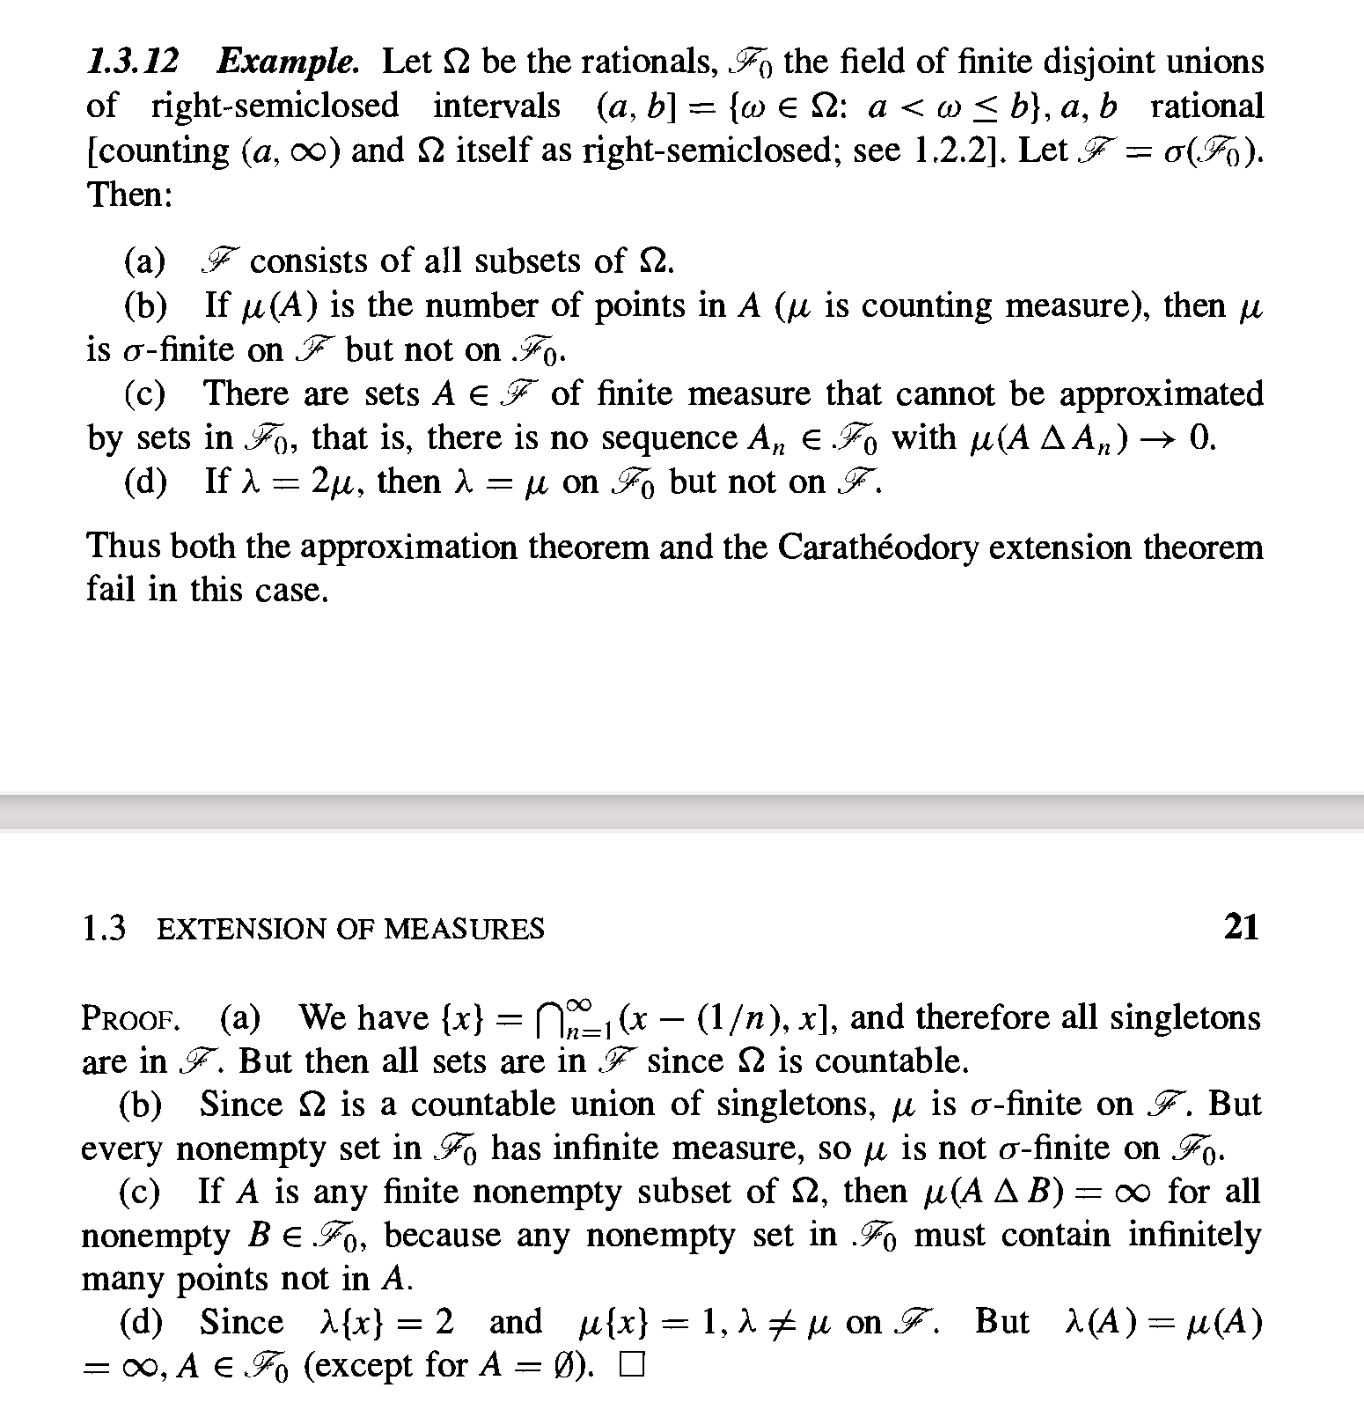
\includegraphics[width=1.\textwidth]{images/example_of_extension}	
\end{figure}
\end{example}

\subsection{Completion of measure spaces}

\begin{definition}
A measure $\mu$ on a $\sigma$-field $\F$ is said to be \textit{complete} iff whenever $A \in F$ and $\mu(A) =0$, we have $B \in F$ for all $B \subset A$.
\end{definition}

\begin{definition}
The \textit{completion} of a measure space $(\Omega, \F, \mu)$ is given by $(\Omega, \F_\mu, \mu)$, where 
\[ \F_\mu := \set{A \cup S : A \in \F, S \subset N 
\text{ for some } N \in \F \text { with } \mu(N) = 0 } \]
and where $\mu$ is extended to $\F_\mu$ by setting $\mu (A \cup S) = \mu(A)$.
\label{def:completion_of_measure_space}
\end{definition}

\begin{remark}
Let us show that Definition \ref{def:completion_of_measure_space} is a valid definition by showing that

\begin{enumerate}
\item \textit{$\F_\mu$ is a $\sigma$-field.}
\item \textit{$\mu$ is a measure on $\F_\mu$.}
\item \textit{The completion is complete.} 	
\end{enumerate}

We justify these in turn:

\begin{enumerate}
\item $\F_\mu$ is closed under countable unions, since 
\[ \cup_{i=1}^\infty (A_i \cup S_i) =  \explaintermbrace{$\in \F$}{(\cup_{i=1}^\infty A_i)} \; \cup \; \explaintermbrace{has measure 0}{(\cup_{i=1}^\infty S_i)} \]
 where the term on the right has measure 0 because $\cup_{i=1}^\infty S_i \subset \cup_{i=1}^\infty N_i \in \F$, and $\mu(\cup_{i=1}^\infty N_i) = \sum_{i=1}^\infty \mu(N_i)= 0$.
 
 $F_\mu$ is also closed under complements, since $S \subset N \implies N^c \subset S^c$, and so
 \[ ( A \cup S)^c = (A^c \cap S^c) = \explaintermbrace{$\in \F$}{(A^c \cap N^c)} \cup \explaintermbrace{has measure 0}{(A^c \cap S^c - N^c)} \]
 where the term on the right has measure 0 by monotonicity, because $A^c \cap S^c - N^c \subset S^c - N^c = S^c \cap (M^c)^c = S^c \cap N \subset N$.
\item First, we show that countable additivity holds in $\F_\mu$. 
\[ \mu(\cupdot_{i=1}^\infty  (A_i \cup S_i)) \stackexplain{see below}{=} \mu(\cupdot_{i=1}^\infty A_i) \stackexplain{$\mu$ countably additive on $\F$ \; }{=} \sum_{i=1}^\infty \mu(A_i) \stackexplain{construction of extension}{=}  \sum_{i=1}^\infty \mu(A_i \cup S_i)  \]
The first equality holds because we can re-represent a disjoint union  $\cupdot_{i=1}^\infty  (A_i \cup S_i) = (\cupdot_{i=1}^\infty A_i) \cup (\cupdot_{i=1}^\infty S_i) $.  Since $\cupdot_{i=1}^\infty S_i  \subset \explaintermbrace{has measure 0 in $\F$}{\cupdot_{i=1}^\infty N_i}$, we have that $\mu((\cupdot_{i=1}^\infty A_i) \cup (\cupdot_{i=1}^\infty S_i)) = \mu(\cupdot_{i=1}^\infty A_i)$. 

Next, we show that $\mu$ is invariant to decompositions: if $A_1 \cup S_1 = A_2 \cup S_2$, then $\mu(A_1 \cup S_1) = \mu(A_2 \cup S_2)$, or more simply $\mu(A_1)=\mu(A_2)$.

\begin{figure}[H]
\centering
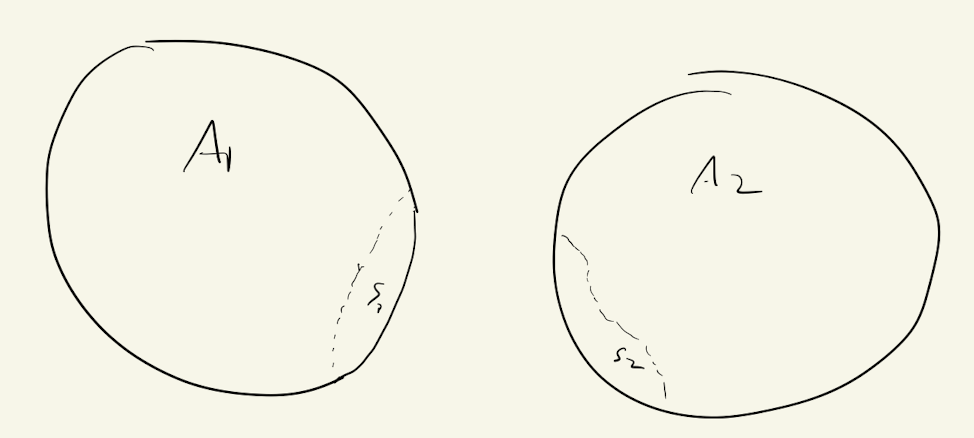
\includegraphics[width=.4\textwidth]{images/completion_of_measure_space}	
\end{figure}

We have    
\[ \mu(A_1)  \stackexplain{countable additivity}{=} \mu(A_1 \cap A_2) + \mu(A_1 \cap A_2^c)\stackexplain{see below}{=} \mu(A_1 \cap A_2) \stackexplain{monotonicity}{\leq} \mu(A_2) \]
where the second equality holds since $A_1 \cap A_2^c \subset S_2$ {\footnotesize (which, in turn, holds since $x \in A_1 \implies x \in A_2 \text{ or } x \in S_2$, so $x \in A_1 \text{ and } x \not\in A_2 \implies x \in S_2$)} .

By symmetry, $\mu(A_2) \leq \mu(A_1)$, so $\mu(A_1)=\mu(A_2)$. 
\item By the definition of a complete measure, we need to show that if $B \in \F_\mu$ and $\mu(B)=0$ then $C \in \F_\mu$ for all $C \subset B$.

%Now $B \in \F_\mu \implies B = \explaintermbrace{$\in \F$}{A} \cup \explaintermbrace{has measure 0}{S}$.  

Now $B \in \F_\mu \implies B = \explaintermbrace{$\in \F$}{A} \cup \explaintermbrace{$\subset N \in \F : \mu(N)=0$}{S}$.  

So our assumption $\mu(B) = 0$ gives us $\mu(A) = 0$, since $\mu(B) = \mu(A \cup S) \stackrel{\text{choice of extension}}{=} \mu(A)  =0$.

Now since we have assumed $C \subset B$ we have
\[\mu(C) \stackexplain{monotonicity}{\leq} \mu(B) \stackrel{B \in \F_\mu}{=} \mu(A \cup S)  \stackexplain{subadditivity}{\leq} \mu(A)+\mu(S)  \stackexplain{see above}{=} 0 + \mu(S) = 0 + 0= 0\]

Since $\mu$ is non-negative, this implies that $\mu(C) =0$.  

We can therefore write $C = \explaintermbrace{$\in \F$}{\emptyset} \cup \explaintermbrace{has measure 0}{C}$, so $C \in \F_\mu$.

Thus, $\mu$ on $\F_\mu$ is complete, since any subset of measure 0 is contained in $\F_\mu$.  
\end{enumerate}
\label{rk:completion_of_measure_space_is_well_defined} 
\end{remark}


 \section{$\S$ 1.4: Lesbesgue-Stieltjes Measures and Distribution Functions} \label{sec:ls_measures_and_distribution_functions}
 
 \begin{definition}
 A \textit{Lesbesgue-Stieltjes measure} on $\R$ is a measure $\mu$ on $\B(\R)$ such that $\mu(I) < \infty$ for each bounded interval $I$.	
 \end{definition}

\begin{definition}
 A \textit{distribution function} on $\R$ is a map $F : \R \to \R$ that is increasing [ $a<b$ implies $F(a) \leq F(b)$] and right continuous [ $\lim_{x \to x_0^+} F(x) = F(x_0)$]. 
 \end{definition}
 
 Here we show that the formula $\mu(a,b] = F(b) - F(a)$ sets up a one-to-one correspondence between distribution functions and Lesbesgue-Stieltjes measures.    Figure \ref{fig:distribution_function_with_positive_mass_on_points_that_is_not_concentrated_on_a_countable_set} helps to illuminate how working with distribution functions allows us to cover both absolutely continuous, discrete, and mixed random variables. 
   
 \begin{figure}[H]
 \centering
 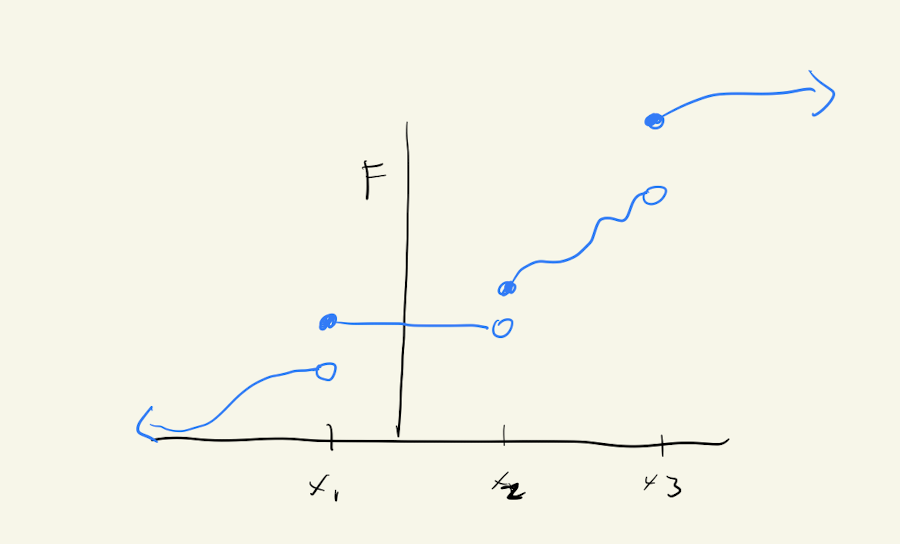
\includegraphics[width=.5\textwidth]{images/distribution_function_with_positive_mass_on_points_that_is_not_concentrated_on_a_countable_set}
 \caption{A distribution function with positive mass on points that is not concentrated on a countable set}	
\label{fig:distribution_function_with_positive_mass_on_points_that_is_not_concentrated_on_a_countable_set}
\end{figure}

   
 
 \subsection{$\S$ 1.4.2 Each Lesbesgue-Stietljes measure uniquely determines a distribution function (up to an additive constant)}
 First, we show that to every Lesbesgue-Stieltjes  measure, there is a unique distribution function (up to an additive constant).  This is the easy part.
 
 \begin{theorem}
 Let $\mu$ be a Lesbesgue-Stietljes measure on $\R$.  Let $\F : \R \to \R$ be defined (up to additive constant) by $F(b)-F(a) = \mu(a,b]$ for $a<b$. Then $F$ is a distribution function.
 \end{theorem}

\begin{proof}
First we show that $F$ is increasing.  We have $F(b) - F(a) = \mu(a,b] \geq 0$, since $\mu$ is non-negative. 

Next we show that $F$ is right continuous.  By the continuity (from above) of measure, 
\[ \ds\lim_{b' \to b+}[F(b') - F(a)] = \ds\lim_{b' \to b+} \mu(a,b'] = \mu(a,b]\]
and continuity from above applies since Lesbesgue-Stietljes measures are finite on any interval.

Thus, rearranging,
\[ \ds\lim_{b' \to b+} F(b') = \mu(a,b] + F(a) = \bigg(F(b)-F(a)\bigg) + F(a) = F(a)\]

\end{proof}


  \subsection{$\S$ 1.4.3-1.4.4 Each distribution function (identified up to additive constant) uniquely determines a Lesbesgue-Stietljes measure }
  
 Now the harder part.  We need to show that every distribution function $F$ (identified up to additive constant) uniquely determines a Lesbesgue-Stieltjes  measure.  
 
 To start, by a similar reasoning as we've seen before (e.g. see Section \ref{sec:extension_and_approximation}), it is straightforward to show that the formula $\mu(a,b] = F(a)-F(b), a,b \in \overline{\R}, a <b$ defines a finitely additive set function on $\F_0(\overline{\R})$, the field of disjoint unions of right semi-closed intervals of the extended reals.  
 
 The challenge will be to show that this set function is countably additive.  If we can do that, then we can apply Carath\'eodory's Extension Theorem to extend this function to $\B(\R)$. 

\begin{lemma}
The set function $\mu$ is countably additive on $\F_0(\overline{\R})$.
\label{lemma:ls_measures_are_countably_additive_on_the_field_of_disjoint_rsc_intervals} 	
\end{lemma}

\begin{proof}
We assume $F(\infty) - F(-\infty) < \infty$, so that $\mu$ is finite.   (We leave the case where $F(\infty) - F(-\infty) = \infty$	to the reader, or see the text.)  Our strategy will be to show that $\mu$ is continuous from above, in which case we can apply Theorem \ref{thm:finite_additivity_plus_continuity_gives_countable_additivity} (b) to show that the set function is countably additive.

Let $A_n$ be a sequence of sets in $\F_0(\overline{\R})$ such that $A_n \downarrow \emptyset$.  Now each $A_n$ is a finite union of disjoint r.s.c. intervals.

\begin{figure}[H]
\centering
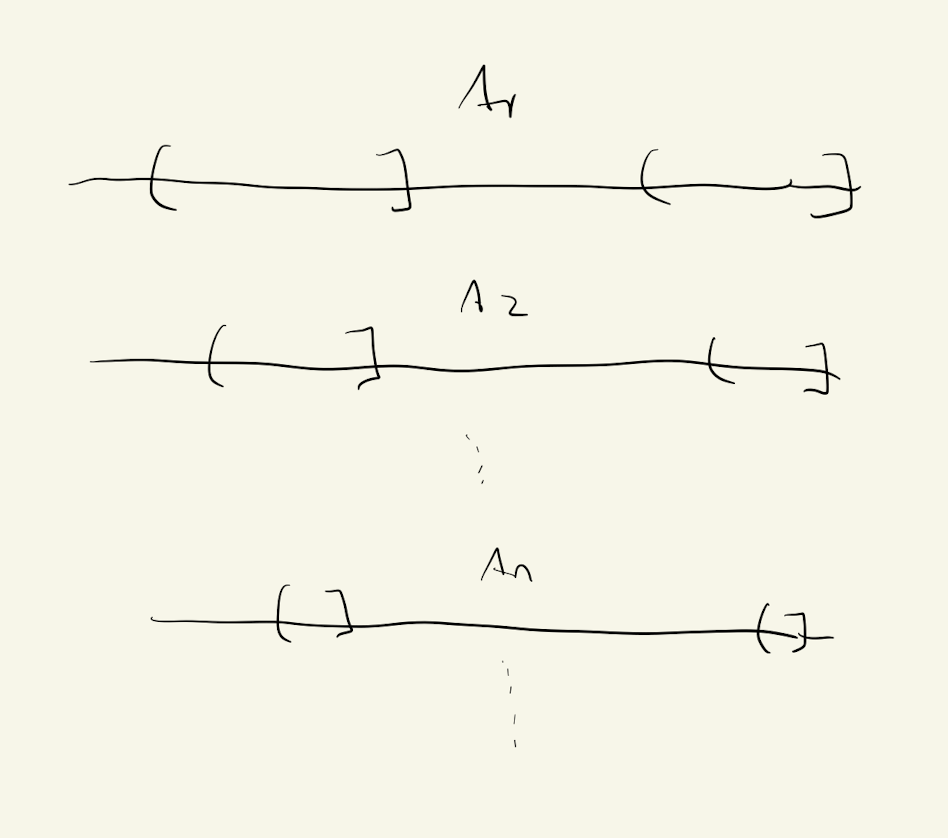
\includegraphics[width=.45\textwidth]{images/decreasing_sequence_of_union_of_rsc_intervals}	
\end{figure}

 Suppose one such interval is $(a,b]$.  By the right continuity of $F$, we can find intervals $(a',b]$ that approximate $(a,b]$ from the inside arbitrarily well, since
\[ \mu(a',b] = F(b) - F(a') \to \mu(a,b] = F(b) - F(a) \text{ as } a' \to a \text{ from the right } \] 
Thus, we can find sets $B_n \in \F_0(\overline{\R})$ whose closures $\overline{B}_n \subset A_n$ and where $\mu(B_n)$ approximates $\mu(A_n)$ to any desired $\epsilon > 0$. 


\begin{figure}[H]
\centering
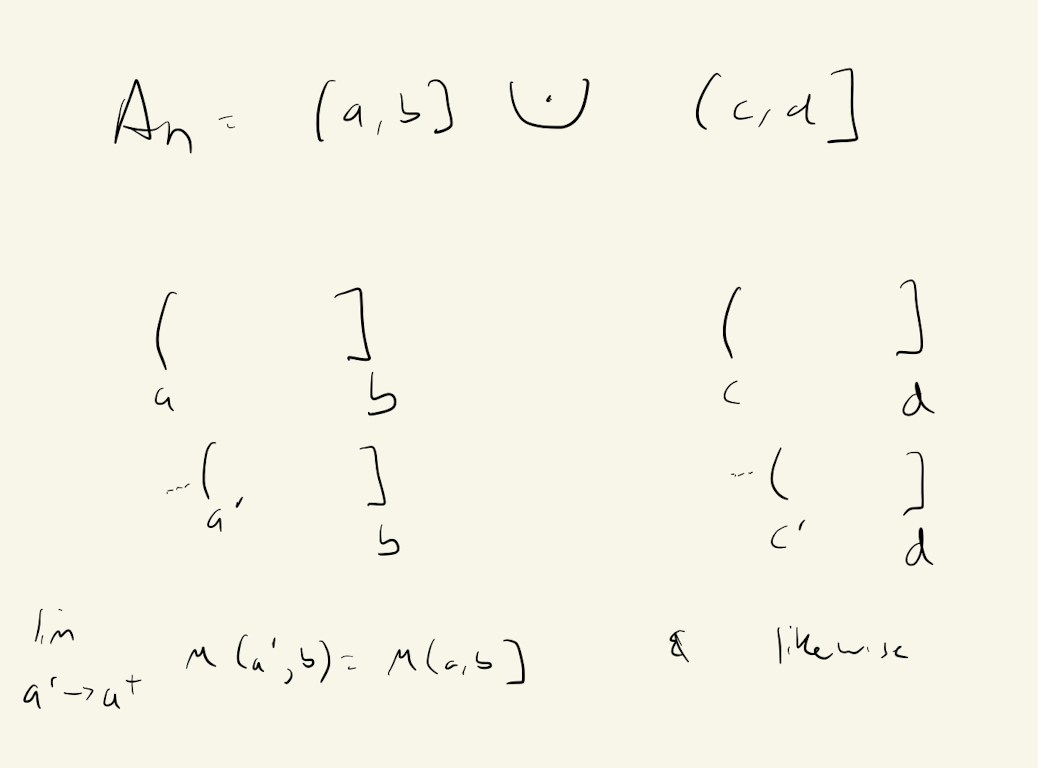
\includegraphics[width=.45\textwidth]{images/approximating_union_of_rsc_intervals}	
\end{figure}

For any fixed $\epsilon>0$, we can choose such a sequence $B_n$ such that $\mu(A_n) - \mu(B_n) < \epsilon 2^{-n} \; (*)$, and we find
\begin{alphabate}
\item $\cap_{n=1}^\infty \overline{B}_n = \emptyset$.	\quad  {[\footnotesize True because each $\overline{B}_n \subset A_n$, so $\cap_{n=1}^\infty \overline{B}_n \subset \cap_{n=1}^\infty A_n = \emptyset$.  ]} 
\item $\cap_{k=1}^n \overline{B}_k = \emptyset$ for sufficiently large $n$.	\quad  {\footnotesize [We have $\overline{\R} \; \stackrel{ \text{item a)}}{=} \; (\overline{\R} - \cap_{n=1}^\infty \overline{B}_n) \; \stackrel{\text{DeMorgan } \eqref{eqn:demorgan_for_relative_complements}}{=} \; \cup_{n=1}^\infty (\overline{\R} - \overline{B}_n)$.   So $\set{\overline{\R} - \overline{B}_n}$ is an open cover of $\overline{\R}$. By the Heine-Borel theorem, there must be a finite subcover.  So for sufficiently large $n$, we have $\cup_{k=1}^n (\overline{\R} - \overline{B}_k) = \overline{\R}$.  Taking complements of both sides, and once again applying DeMorgan's law \eqref{eqn:demorgan_for_relative_complements} to the relative complement, we find $\cap_{k=1}^n \overline{B}_k = \emptyset$.  ]}
\end{alphabate}

So now we use a piece-and-difference decomposition (Theorem \ref{thm:basic_properties_of_finitely_additive_set_functions} (b) ):
\begin{align*}
A_n &= \bigg( \bigcap_{k=1}^n B_k \bigg) \; \bigcupdot \; \bigg(  A_n - \bigcap_{k=1}^n B_k \bigg) \\
\implies \mu(A_n) &= \cancelto{0}{\mu(\cap_{k=1}^n B_k)} \; + \; \mu(A_n - \cap_{k=1}^n B_k) && \tinytext{countable additivity; item b) above}\\ 
& \stackrel{1}{\leq} \mu( \cup_{k=1}^n (A_k - B_k))&& \tinytext{monotonicity} \\
& \leq \sum_{k=1}^n \mu( A_k - B_k) && \tinytext{finite subadditivity} \\
& = \sum_{k=1}^n \mu( A_k) - \mu(B_k) && \tinytext{piece-and-difference decomposition; also uses finiteness} \\
&\leq \epsilon \sum_{k=1}^n 2^{-k} \\
& < \epsilon. 
\end{align*}
where the monotonicity property in (1) applies because $A_n - \cap_{k=1}^n B_k \stackrel{\text{DeMorgan}}{=} \cup_{k=1}^n
(A_n - B_k) \subset \cup_{k=1}^n
(A_k - B_k)$.

In summary, we have seen that for any fixed $\epsilon >0$, we have $\mu(A_n) < \epsilon$ for sufficiently large $n$. Thus, $\mu(A_n) \to 0$, and so $\mu$ is continuous from below.  So by Theorem \ref{thm:finite_additivity_plus_continuity_gives_countable_additivity} (b), $\mu$ is countably additive.
\end{proof}

\begin{remark}
The proof of Lemma \ref{lemma:ls_measures_are_countably_additive_on_the_field_of_disjoint_rsc_intervals} is a very cool application of Heine-Borel!  In trying to show continuity from above, we started out with an \textit{infinite} intersection of sets.  But in showing that the measure of the sequence converged, we needed to work with \textit{finite} collection so that we could apply \textit{finite} subadditivity, since that's all we had to use, by assumption. 
\end{remark}

 
\bibliography{references_ash_notes.bib}
\bibliographystyle{unsrt}

\appendix

\section{Appendix}
\subsection{Right semi-closed intervals}
\begin{definition}
A \textbf{right semi-closed interval} is a set of the form $(a,b] = \set{x : a < x \leq b}, -\infty \leq a < b < \infty$.  By convention, we also count $(a,\infty)$ as right semi-closed for $-\infty \leq a < \infty$. 
\label{def:rsc_intervals}
\end{definition}

\subsection{DeMorgan's Law applies to relative complements} 

\begin{remark}
DeMorgan's Law also holds for relative complements.  That is, given a sequence of sets $A_1, A_2, ...$ that are subsets of another set $X$, we have:

\begin{align*}
X - \bigcap_{n=1}^\infty A_n = \bigcup_{n=1}^\infty (X - A_n)
\labelit \label{eqn:demorgan_for_relative_complements}	
\end{align*}

	
\end{remark}


\end{document}
